\documentclass{../../fal_assignment}
\graphicspath{ {../../} }

\usepackage{amsmath}
\usepackage{enumitem}
\setlist{nosep} % Make enumerate / itemize lists more closely spaced
\usepackage[T1]{fontenc} % http://tex.stackexchange.com/a/17858
\usepackage{url}
\usepackage{todonotes}
\usepackage{algorithm}
\usepackage{algpseudocode}

\usepackage{listings}
\lstset{
	basicstyle=\ttfamily,
	frame=single,
	showstringspaces=false,
	breaklines=true,
	prebreak={\space\hbox{\textcolor{gray}{$\hookleftarrow$}}}
}
\lstset{
	commentstyle=\ttfamily\textit,
	keywordstyle=\ttfamily\textbf,
	stringstyle=\ttfamily,
	rulecolor=\color{black}
}
\lstset{language=C++}

\usepackage{tikz}
\usetikzlibrary{shapes.geometric, arrows}
\tikzstyle{flowchartnode} = [rectangle, minimum height=0.8cm, text centered, text width=3cm, draw=black, font=\small]
\tikzstyle{startstop} = [flowchartnode, rounded corners=0.4cm]
\tikzstyle{process} = [flowchartnode]
\tikzstyle{io} = [flowchartnode, trapezium, trapezium left angle=70, trapezium right angle=110, text width=2cm]
\tikzstyle{decision} = [flowchartnode, diamond, aspect=2, text width=2cm]
\tikzstyle{arrow} = [thick,->,>=stealth]

\title{Worksheet A: Introduction to C++}
\module{COMP130}
\author{Dr Ed Powley}

\begin{document}

\maketitle

\section*{Introduction}

\begin{marginquote}
``War. War never changes.''

--- The Narrator, Fallout
\end{marginquote}
\marginpicture{flavour_pic}{
    The terminal hacking minigame in \emph{Fallout 4}.
}

The open-world RPG \textbf{Fallout~4} contains a terminal hacking minigame, in which
the player must guess a secret $n$-letter word.
In COMP110 Worksheet~B, you modelled this minigame using a flowchart and a piece of pseudocode.
In this worksheet, you will implement the minigame as a C++ console application.

In the minigame, each guess receives a \textbf{likeness} score,
defined as the number of letters which match the secret word (i.e.\ the same letter in the same position).
For example if the secret word is \texttt{HOUSE} and the guess is \texttt{MOUSE}, the likeness is $4$ out of $5$.
If the guess is \texttt{HOPES}, the likeness is $2$ out of $5$
(the letters \texttt{S} and \texttt{E} do not count as they are in the wrong positions).
The minigame ends when the player guesses correctly, or after four incorrect guesses.
(In Fallout~4 there is a way to replenish the number of available guesses,
but this is disregarded in this worksheet for simplicity.)

Algorithm~\ref{alg:a_likeness} gives pseudocode for calculating the likeness between a guessed word and the secret word.
Figure~\ref{fig:flowchart_a} shows a flowchart for the overall game.

To complete this worksheet:
\begin{enumerate}[label=(\alph*)]
	\item \textbf{Implement} Algorithm~\ref{alg:a_likeness} as a C++ function.
		The function should take two \lstinline{std::string}s as arguments, and return an \lstinline{int}.
	\item \textbf{Complete} the provided template program so that it implements the logic
		shown in Figure~\ref{fig:flowchart_a}.
\end{enumerate}

\begin{algorithm}[h]
\begin{algorithmic}
    \Procedure{GetLikeness}{guessedWord, secretWord}
        \State $\text{result} \gets 0$
        \For{$i = 0, 1, \dots, \text{secretWord.length} - 1$}
            \If{$\text{secretWord}[i] = \text{guessedWord}[i]$}
                \State increment result
            \EndIf
        \EndFor
        \State \textbf{return} result
    \EndProcedure
\end{algorithmic}
\caption{An algorithm for calculating the likeness score for the terminal hacking minigame.}
\label{alg:a_likeness}
\end{algorithm}

\section*{Submission instructions}

Begin by \textbf{forking} the GitHub repository at the following URL:

\url{https://github.com/Falmouth-Games-Academy/comp130-worksheets}

The \url{worksheet_A} directory contains a Visual C++ project to build upon.
\textbf{Read} and \textbf{understand} the provided code.
\textbf{Add} code to satisfy the requirements listed above.
You may make any changes to the provided code that you see fit,
and may add new files to the project,
however please do \textbf{not} move or rename the project or the existing files.

Attend the timetabled COMP130 session in \textbf{week commencing 23rd January 2017},
ensuring that you have uploaded all material to GitHub before this time.

\section*{Marking criteria}

Remember that \textbf{it is better to submit incomplete work than to submit nothing at all}.
Any attempt, even unfinished, will receive a passing grade.

Your work will be marked according to the following criteria:
\begin{itemize}
	\item \textbf{Functional coherence}. Is your implementation correct and free of obvious bugs?
		Does it adhere to the specification outlined in this worksheet?
	\item \textbf{Sophistication}. Have you made use of appropriate code structures and data structures?
		Note the emphasis is on \textbf{appropriate}; extra credit will \textbf{not} be given for unnecessarily complex solutions.
	\item \textbf{Maintainability}. Is your code well commented? Are your identifier names appropriate and descriptive?
		Have you adhered to appropriate coding standards?
\end{itemize}

\clearpage
\newgeometry{margin=1.5cm}
\begin{figure}
\begin{center}
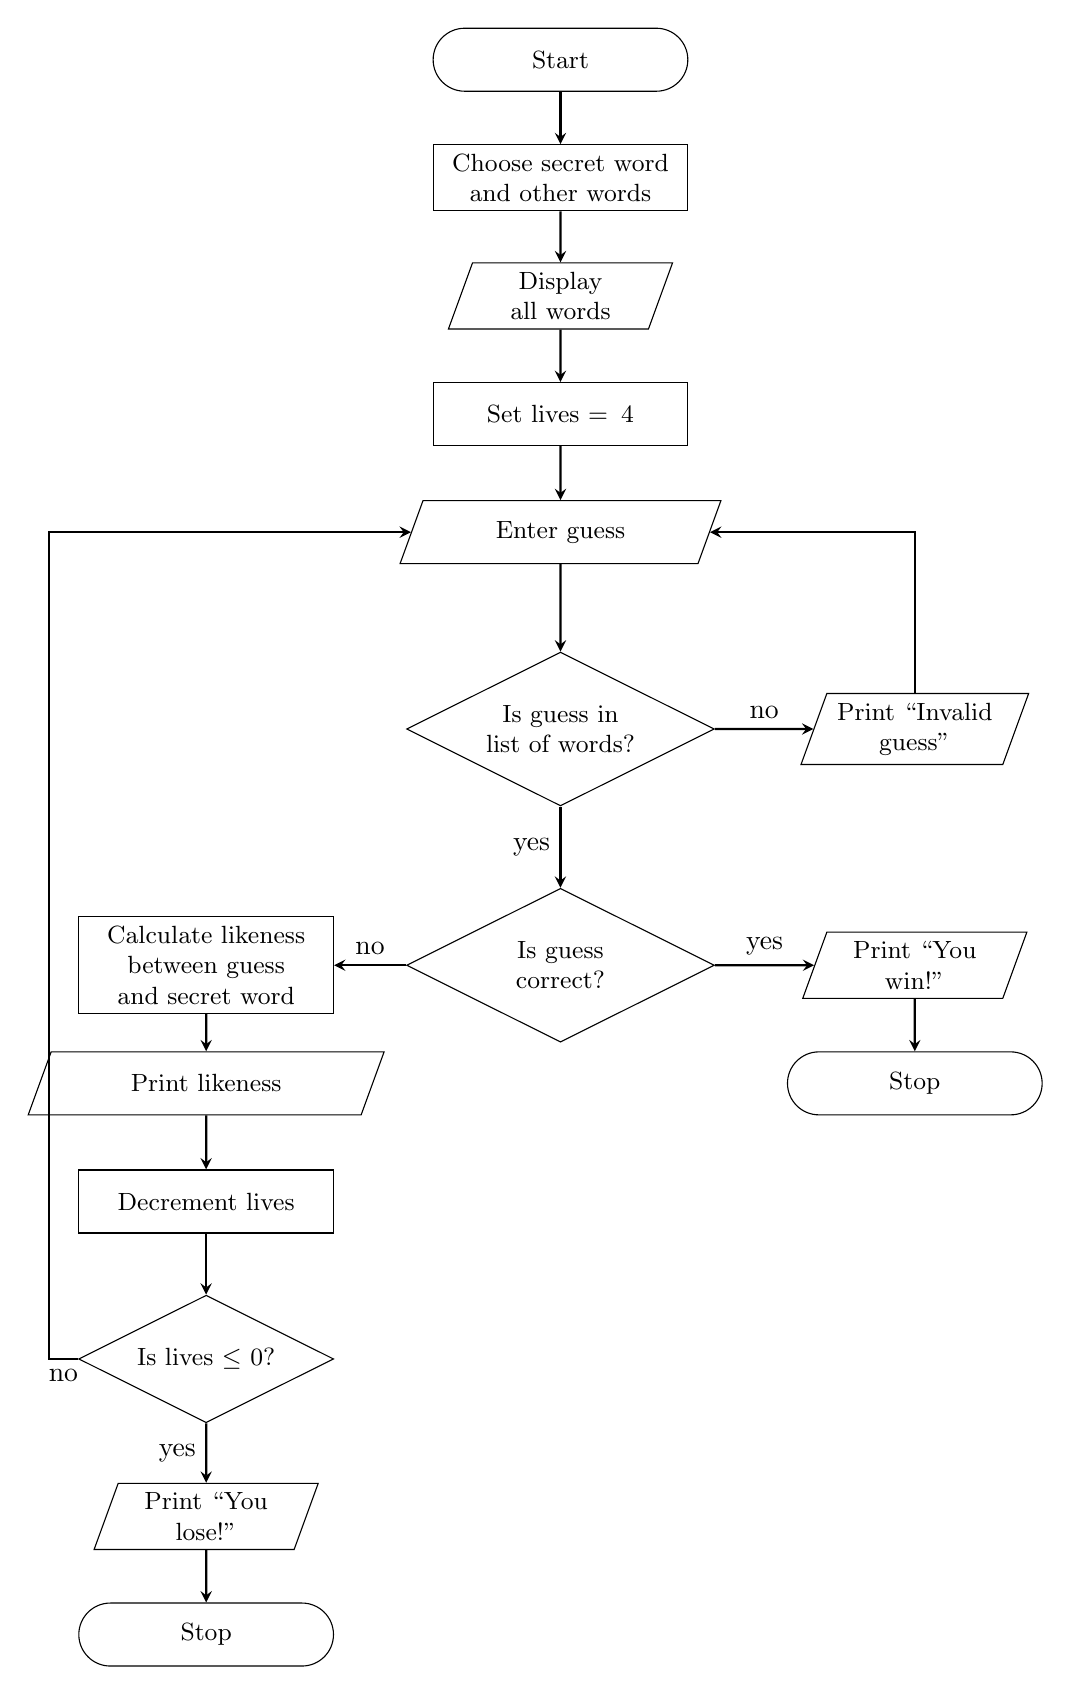
\begin{tikzpicture}[node distance=1.5cm]
\node (start) [startstop] {Start};
\node (choosewords) [process, below of=start] {Choose secret word and other words};
\node (displaywords) [io, below of=choosewords] {Display all words};
\node (initlives) [process, below of=displaywords] {Set lives $= 4$};
\node (enterguess) [io, below of=initlives] {Enter guess};
\node (isguessvalid) [decision, below of=enterguess, yshift=-1cm] {Is guess in list of words?};
\node (guessinvalid) [io, right of=isguessvalid, xshift=3cm] {Print ``Invalid guess''};
\node (isguesscorrect) [decision, below of=isguessvalid, yshift=-1.5cm] {Is guess correct?};
\node (youwin) [io, right of=isguesscorrect, xshift=3cm] {Print ``You win!''};
\node (stopwin) [startstop, below of=youwin] {Stop};
\node (calclikeness) [process, left of=isguesscorrect, xshift=-3cm] {Calculate likeness between guess and secret word};
\node (showlikeness) [io, below of=calclikeness] {Print likeness};
\node (loselife) [process, below of=showlikeness] {Decrement lives};
\node (isdead) [decision, below of=loselife, yshift=-0.5cm] {Is lives $\leq 0$?};
\node (youlose) [io, below of=isdead, yshift=-0.5cm] {Print ``You lose!''};
\node (stoplose) [startstop, below of=youlose] {Stop};
\draw [arrow] (start) -- (choosewords);
\draw [arrow] (choosewords) -- (displaywords);
\draw [arrow] (displaywords) -- (initlives);
\draw [arrow] (initlives) -- (enterguess);
\draw [arrow] (enterguess) -- (isguessvalid);
\draw [arrow] (isguessvalid) -- node[anchor=south] {no} (guessinvalid);
\draw [arrow] (guessinvalid) |- (enterguess);
\draw [arrow] (isguessvalid) -- node[anchor=east] {yes} (isguesscorrect);
\draw [arrow] (isguesscorrect) -- node[anchor=south] {yes} (youwin);
\draw [arrow] (youwin) -- (stopwin);
\draw [arrow] (isguesscorrect) -- node[anchor=south] {no} (calclikeness);
\draw [arrow] (calclikeness) -- (showlikeness);
\draw [arrow] (showlikeness) -- (loselife);
\draw [arrow] (loselife) -- (isdead);
\draw [arrow] (isdead) -- node[anchor=east] {yes} (youlose);
\draw [arrow] (youlose) -- (stoplose);
\coordinate[left of=isdead, xshift=-0.5cm] (tmp1);
\draw [arrow] (isdead) -- node[anchor=north] {no} (tmp1) |- (enterguess);
\end{tikzpicture}
\end{center}
\caption{Flowchart for the Terminal Hacking game}
\label{fig:flowchart_a}
\end{figure}

\end{document}
